\section{Metoda triangulacji laserowej}
Wśród urządzeń korzystających z metody triangulacji laserowej można wyróżnić dwa podstawowe typy. W pierwszym typie takiego skanera układ pomiarowy składa się z nadajnika laserowego, obiektu pomiarowego oraz kamery. Poprzez przesuwanie wiązki po nieruchomym obiekcie, znając położenie kamery oraz korzystając z odpowiednich wzorów można wyznaczyć położenie zmierzonych punktów w docelowym układzie współrzędnych \cite{mikulski2013metody}. Zaletami tej konstrukcji są dokładność i wysoka rozdzielczość \cite{nowacki2018pomiar}. Skanery te jednak nie sprawdzają się przy rekonstrukcji błyszczących oraz przezroczystych powierzchni. Zasada działania skanera została przedstawiona na rysunku ~\ref{fig:triangPic}. 

\begin{figure}[H]
  \centering
%   \includesvg[scale=0.75]{trianSVG}
    \includesvg[scale=0.6]{skanerTriaSvgNowy}
  

  \caption{Schemat skanera wykorzystującego triangulację laserową \cite{mikulski2013metody}.}   
  \label{fig:triangPic}
\end{figure}
\newpage 
Posługując się poniższymi wzorami można uzyskać współrzędne przestrzenne mierzonego obiektu, co w rezultacie pozwala na jego odwzorowanie w komputerowej symulacji:

\begin{equation}
    \begin{aligned} 
    \begin{cases}
        & \ X=d+x_{wyn} \\
      & Y=k_{y}\cdot y_{pic} \\ 
      & Z=ctg(\beta) \cdot x_{wyn}\\
      &  x_{wyn}=k_{x}\cdot x_{pic}\\ 
    \end{cases}
            
    \end{aligned}
\end{equation}

\noindent Zmierzony obiekt posiada współrzędne X,Y,Z. Kamera jest oddalona od podstawy ramienia uchwytu o odległość d. Wynik pomiaru w kierunku osi X w docelowych jednostkach miary został oznaczony poprzez $x_{wyn}$. Linia lasera tworzy z płaszczyzną obrazu kąt $\alpha$. Współrzędne linii lasera odczytane przez kamerę oznaczone są jako $x_{pic},y_{pic}$. W celu przejścia na docelowe jednostki miary należy użyć odpowiedniej skali przejścia dla obu współrzędnych X oraz Y, odpowiednio $k_{x}$ i $k_{y}$.\\
\indent Drugi typ skanerów opartych o metodę triangulacji laserowej steruje położeniem obiektu względem lasera. Korzystając z tego rozwiązania, możliwe jest odwzorowanie bardziej skomplikowanych kształtów. W skład elementów konstrukcyjnych takiego układu wchodzą laser, kamera oraz tacka obrotowa z umieszczonym na niej obiektem pomiarowym.
W przeciwieństwie do skanera pierwszego typu, w tym układzie kamera oraz laser są nieruchome. Porusza się jedynie tacka obrotowa z obiektem. Laser wyświetla pionową linię na obiekt, a kamera rejestruje ten obraz. Tacka obracana jest o stały kąt $\Delta \theta$. Po zmierzeniu kąta nachylenia α pomiędzy kamerą, a laserem jak również kąta nachylenia β kamery względem tacki, można dokonać transformacji ze współrzędnych obiektu do współrzędnych obrazu przechodzących przez oś obrotu podstawy. Schemat działania takiego urządzenia został przedstawiony na rysunku ~\ref{fig:triangPic2}.

\begin{figure}[H]
  \centering 
    \includesvg[scale=0.45]{skanPionSv.svg}  

  \caption{Układ współrzędnych nieruchomego skanera \cite{mikulski2013metody}.}   
  \label{fig:triangPic2}
\end{figure}
\newline
Współrzędne zmierzonego obiektu w układzie kamery można opisać poniższymi równaniami. Przedstawiają one sposób na przejście ze współrzędnych obiektu do współrzędnych kamery.

\begin{equation}
    \begin{aligned}
    \begin{cases}
        & \ Z_{doc}=y_{0}-(y-(x_{las}-x_{0}))tan(a) \\
          & X_{doc}=x-x_{0}+(y_{las}-y_{0})tan(\beta) \\
          & Y_{doc}=0\\
        \end{cases}
        
        \end{aligned}
\end{equation}

Wartości X oraz Y są współrzędnymi obrazu kamery w pikselach. $X_{las},Z_{las}$ są współrzędnymi układu linii emitowanej przez laser. Kąt nachylenia linii laserowej do płaszczyzny obrazu symbolizuje wartość $\alpha$. Układ docelowy nachylony jest do płaszczyzny obrazu pod kątem $\beta$. Środek tacki obrotowej przedstawionej na obrazie kamery ma współrzędne $x_{0},y_{0}$ w pikselach. Docelowy układ współrzędnych określają współrzędne $X_{doc},Y_{doc},Z_{doc}$.\\
\indent Ostatecznie korzystając z macierzy obrotu względem osi $Z_{doc}$ można uzyskać współrzędne chmury punktów.

\begin{equation}
    \begin{aligned}
    \begin{cases}
        & \ X_{pkt}=X_{doc}\cdot cos(\theta)-Y_{doc}\cdot sin(\theta) \\
          & Y_{pkt}=X_{doc}\cdot sin(\theta)+Y_{doc}\cdot cos(\theta) \\
          & Z_{pkt}=Z_{doc}
        \end{cases}
        
        \end{aligned}
\end{equation}
gdzie: $\theta$ przedstawia kąt obrotu tacki, $X_{doc},Y_{doc},Z_{doc}$ są współrzędnymi układu kamery, natomiast $X_{pkt},Y_{pkt},Z_{pkt}$ określają współrzędne w układzie chmury punktów względem środka tacki.\\
\indent Na rynku istnieje wiele skanerów trójwymiarowych wykorzystujących metodę triangulacji laserowej. Poniżej zostaną omówione charakterystyki jednego z nich. Charakterystyki jakości pomiaru skanera Faro Focus zostały przedstawione w tabeli ~\ref{tab:faroCharTab}.


\begin{table}[H]
\begin{center}
\caption{\label{tab:faroCharTab}Charakterystyki skanera Faro Focus S350 \cite{farofocusDatasheet}.}
\begin{tabular}{ |c| c| }
 \hline
 {\small Zasięg} & {\small 0.6 m-350 m}\\ 
  \hline
 {\small Błąd pomiaru odległości} & {\small $\pm$1 mm}\\  
 \hline
 {\small Prędkość pomiaru} & {\small do 976000 $\frac{pkt}{s}$ }\\  
  \hline
 {\small Dokładność kątowa} & {\small Do 19 sekund kątowych}  \\  
  \hline
  {\small Dokładność pozycji 3D} & {\small 3.5 mm}  \\  
  \hline
     {\small Długość fali lasera } & {\small 1550 nm}  \\  
  \hline
\end{tabular}
\end{center}
\end{table}
Metoda triangulacji laserowej umożliwia mierzenie dużych obiektów z dalekiej odległości. Dlatego też znajduje ona zastosowanie na przykład w budownictwie. Dzięki niej inżynierzy pracujący przy konstrukcjach są w stanie skanować pełnowymiarowe budynki, a następnie dokonywać ich oględzin w postaci cyfrowej. Niestety jednak pomiar o wysokiej rozdzielczości zajmuje znacznie więcej czasu niż przy wykorzystaniu innych metod pomiarowych.Jest to spowodowane zależnością, iż czas pomiaru obiektu jest proporcjonalny do rozdzielczości kątowej skanera. To znaczy, że wraz ze wzrostem rozdzielczości kątowej rośnie również czas pomiaru, co zostało zobrazowane na rysunku ~\ref{fig:lasertriangchart}.
\begin{figure}[H]
  \centering
  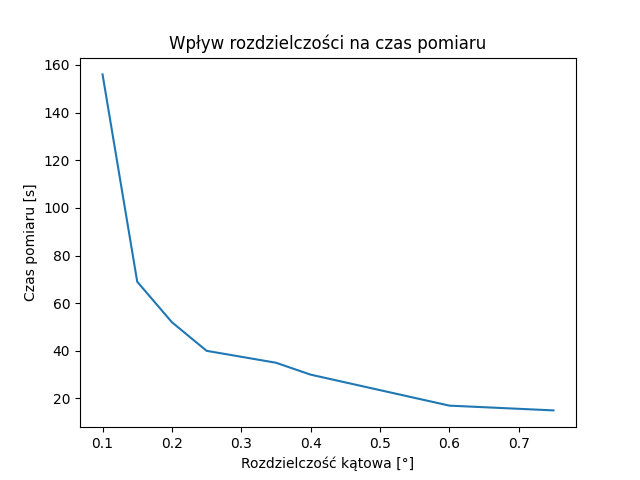
\includegraphics[scale=0.6]{wplywRozdzielczosci.png}
  \caption{Czas pomiaru w zależności od dokładności pomiaru \cite{el2008integrating}.}   
  \label{fig:lasertriangchart}
\end{figure}